%% Here we give a brief introduction about the scope and importance of aligning the muon  
%% detectors, describe the DT and CSC geometries (or give a reference to papers where they are  
%% described in detail), define the global and local coordinate systems and define any  
%% conventions used.  
 
%% The approximate length is one page plus one to three figures showing the 
%% CSC and DT geometries and the coordinate systems. 

The CMS experiment~\cite{ref:cms} features a large muon tracking system for
identifying muons and reconstructing their momenta.  As with all
tracking systems, the momentum resolution of reconstructed tracks depends both
on the intrinsic position resolution of its detector elements and on their
alignment.  By ``alignment,'' we mean measurement of the detector
elements' positions and orientations in space, 3 translational plus 3
rotational degrees of freedom, knowledge which allows us to transform
hit positions from detector-bound local coordinate systems into a
common coordinate system for all CMS tracking systems.

This paper describes methods for aligning barrel Drift Tube (DT)
chambers and endcap Cathode Strip Chambers (CSC) and their internal
layers with tracks, as well as results of alignments using cosmic rays
from the 2008 Cosmic Run at Four Tesla (CRAFT) exercise
and beam-halo tracks from the 2008 LHC injection.  We will consider two
cases: (1) alignment relative to the modular structures from which the
muon system is built, and (2) alignment in a single coordinate system
defined by the central CMS tracker.  Alignment using integrated
physical measurement devices such as lasers, rulers, and
inclinometers is described elsewhere~\cite{ref:hardware_alignment}, as
are the details of the data transfer and computing model which is used
to implement these algorithms~\cite{ref:workflow}.

The scale of desired alignment precision is given by the intrinsic
resolution of the chambers: 100--300~$\mu$m.  Since alignment errors
and measurement errors add in quadrature, misalignment becomes
irrelevant once it is significantly below the intrinsic hit
resolution.

\subsection{Geometry of the muon system}

The muon system is a collection of independent tracking chambers, each
of which contains parallel measurement planes, here called chamber layers.  The
chambers are mounted on 5 moveable barrel wheels (labeled $-$2 through
$+$2) and 6 endcap disks (3 per endcap).  Within these large
structures, chambers are arranged in stations, labeled in
Figure~\ref{fig:muon_system_labeled}, with azimuthal positions called
sectors (in the barrel) or simply chamber number (in the endcap).  Barrel
stations 1--3 have 12 sectors, station 4 has 14 sectors, and most
rings of chambers in the endcap have 36 chambers, the exceptions being
ME2/1, ME3/1, and ME4/1, which have 18.

\begin{figure}
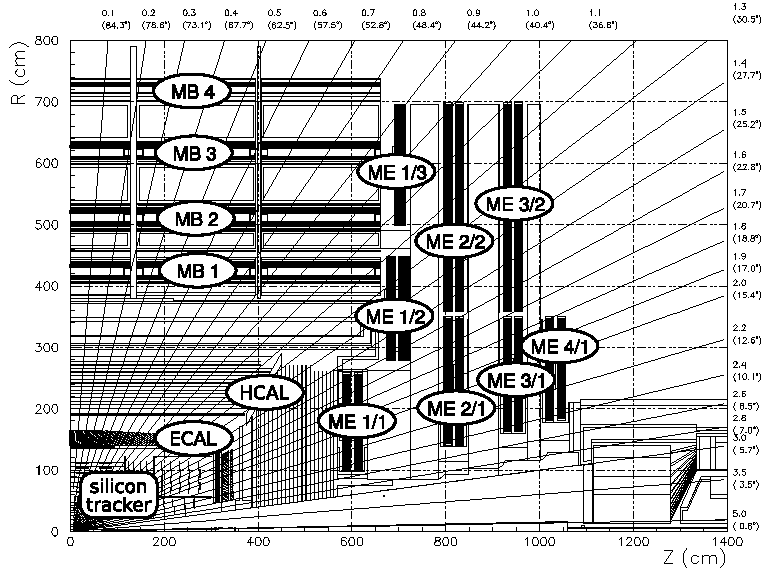
\includegraphics[height=\linewidth, angle=90]{plots/intro_geom/muon_system_labeled.pdf}

\caption{A quarter-view of CMS with labeled muon barrel (MB) and endcap (ME) stations. \label{fig:muon_system_labeled}}
\end{figure}

Barrel DT chambers have internal structure: superlayers
containing 4 layers each.  Stations 1--3 have 3 superlayers, the
middle one measuring a direction orthogonal to the outer
two.  Station 4 chambers have no middle superlayer (only superlayers~1
and 3).  Endcap CSCs contain 6 identical layers, each of which
measures both coordinates with intersecting cathode strips and anode
wires.

\subsection{Coordinate systems and conventions}

The Alignment Integration Frame, a coordinate system in which all
tracking systems are to be aligned, is defined by the 
tracker.  The origin of this system is the center of mass of the
tracker's detector elements~\cite{ref:tracker_alignment}, close to the
LHC interaction point, and oriented such that the $+z$ axis points
roughly along the beamline, to the west.  The $+y$ axis points
vertically upward, with $+x$ forming a right-handed coordinate system
by pointing south~\cite{ref:twikiCMSConventions}.  These same
coordinates can be expressed cylindrically, with $x$ and $y$ replaced
by $r = \sqrt{x^2 + y^2}$ and $\phi = \tan^{-1}(y/x)$.  The
curvilinear coordinate $r\phi$ is perpendicular to the beamline and
to rays from the beamline, and differentials of $r\phi$ are understood to
vary in $\phi$, not $r$ (so $d(r\phi)$ is equivalent to $r \, d\phi$).

Each muon chamber and layer has its own local coordinate system,
centered on the subdetector with local $z$ being perpendicular to the
measurement planes, and $+z$ points in the direction of decreasing
layer number.  The local $x$ axis roughly corresponds to global $r\phi$ (though for some chambers the direction is reversed),
and local $y$ forms a right-handed coordinate system.  In the absence
of misalignment, $y$ is parallel to the beamline for DT chambers and
radial for CSCs.

Layer/superlayer coordinate systems differ slightly from their parent
chambers.  The origin of each coordinate system is centered such that
$z=0$ lies on the layer and the average of layers in the superlayer, and
both layers and superlayers have small offsets in $x$ as well.  The
middle superlayer of DT chambers (superlayer~2) are rotated by 90$^\circ$ with
respect to the chamber coordinates, such that $x$ measurements in
these layers are $y$ positions in chamber coordinates.  Internal
alignments of layers introduce additional corrections.

Cathode strips in CSC layers fan radially from the beamline,
intersected by anode wires.  The strips measure a coordinate
perpendicular to their orientation, which in the absence of
misalignment coincides with global $r\phi$ throughout the chamber.  We
find ``local $r\phi$,'' or local $x$ times the cosine of the strip
angle, to be a more convenient coordinate than $x$ for CSCs.  This is
because local $r\phi$ is determined purely by high-precision strip
measurements, avoiding input from the groups of ganged wires which
would introduce a complicated and large-scale (cm) granularity to the
residuals distributions.

We describe the orientations of chambers and layers with $\phi_x$,
$\phi_y$, and $\phi_z$, where each is a right-hand rotation around the
corresponding coordinate axis.  The 3-D rotation is the following
composition:
\begin{equation}
\left(\begin{array}{c c c}
1 & 0 & 0 \\
0 & \cos\phi_x & \sin\phi_x \\
0 & -\sin\phi_x & \cos\phi_x
\end{array}\right) \cdot 
\left(\begin{array}{c c c}
\cos\phi_y & 0 & -\sin\phi_y \\
0 & 1 & 0 \\
\sin\phi_y & 0 & \cos\phi_y
\end{array}\right) \cdot
\left(\begin{array}{c c c}
\cos\phi_z & \sin\phi_z & 0 \\
-\sin\phi_z & \cos\phi_z & 0 \\
0 & 0 & 1
\end{array}\right)\mbox{.}
\end{equation}

